\documentclass[12pt]{article}
\usepackage[spanish]{babel}
\usepackage[utf8]{inputenc}
\usepackage{amsmath}
\usepackage{graphicx}
\usepackage{pdfpages}
\usepackage{listings}

\lstdefinestyle{Haskell}{
  language=Haskell,
  tabsize=2,
  showspaces=false,
  showstringspaces=false,
  frame=single,
  breaklines,
  breakatwhitespace,
  basicstyle=\small
}

\begin{document}

\begin{titlepage}

\newcommand{\HRule}{\rule{\linewidth}{0.5mm}}

\center

\textsc{\LARGE Universidad de Buenos Aires}\\[1.5cm]


\includegraphics{docs/images/logo-fiuba.png}\\[1cm]

\textsc{\Large Facultad de Ingeniería}\\[0.5cm]
\textsc{\large (75.31) Teoría de Lenguaje}\\[0.5cm]
{\large 1\textsuperscript{er} Cuatrimestre 2015}\\[0.5cm]

\HRule \\[0.4cm]
{ \huge \bfseries Ejercicios Adicionales Haskell}\\[0.4cm]
\HRule \\[1.5cm]

\large Andrés Arana, P.86203

\vfill

\end{titlepage}

\begin{abstract}

El presente informe se sumarizan las soluciones a los diferentes problemas
planteados como trabajo compensatorio por ausencias de la materia (75.31)
Teoría de Lenguaje.

\end{abstract}

\tableofcontents

\clearpage

\section{Ejercicios Adicionales}

\subsection{Filas impares y columnas pares}

\lstinputlisting[style=Haskell]{sources/haskell/e01.hs}

\subsection{Índice de sublista}

\lstinputlisting[style=Haskell]{sources/haskell/e02.hs}

\subsection{Profundidad de una lista}

No se encontró forma de representar, usando el sistema de tipos del lenguaje,
una lista heterogénea como la que se plantea como entrada de la función. Las
listas estándar de Haskell son homogéneas, por lo que todos los elementos deben
tener el mismo tipo. No se puede representar, con las listas estándar de
Haskell, una lista de números o listas, ni una lista de listas de distintos
tipos.

\subsection{Programación de alto orden}

\subsubsection{Paridad}

\lstinputlisting[style=Haskell]{sources/haskell/e04a.hs}

\subsubsection{Suma de cuadrados}

\lstinputlisting[style=Haskell]{sources/haskell/e04b.hs}

\subsubsection{Subsecuencias}

\lstinputlisting[style=Haskell]{sources/haskell/e04c.hs}

\subsubsection{Frente a par}

\lstinputlisting[style=Haskell]{sources/haskell/e04d.hs}

\subsection{Tipo algebráico de polinomios}

\lstinputlisting[style=Haskell]{sources/haskell/e05.hs}

\clearpage
\appendix

\section{Enunciado}

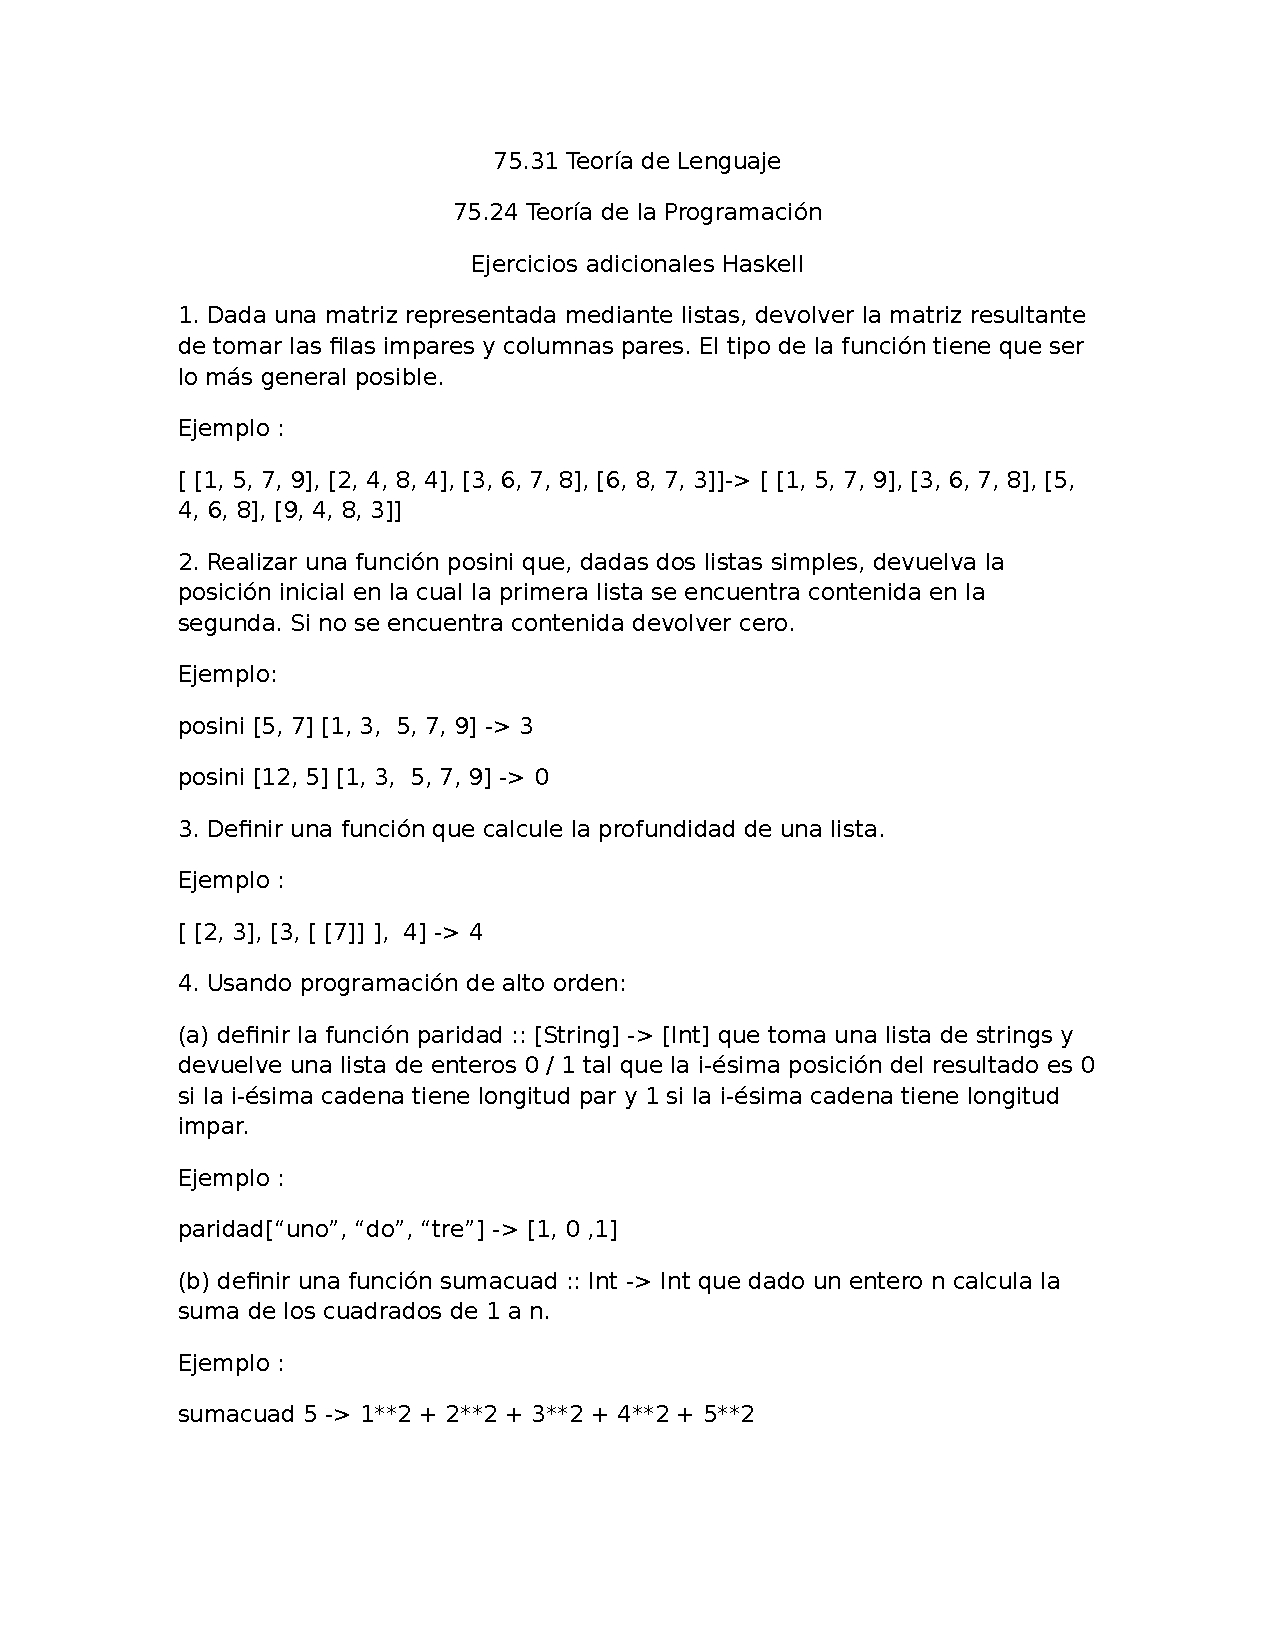
\includepdf[pages=-,scale=.75,pagecommand={}]{docs/enunciados/adicionales-haskell.pdf}

\end{document}
